\problemname{}

\illustration{0.3}{image.png}{
    CC BY-SA 4.0 by gankogroup on \href{https://www.vecteezy.com/vector-art/4546680-vector-illustration-of-silhouette-alcohol-bottle}{vecteezy}
}

% optionally define variables/limits for this problem
\newcommand{\maxn}{10^{18}}

En tant que président du KARWA, le fameux Klan des Assoiffés Rassemblés pour le Whisky et l'Apéro, vous vous retrouvez avec une montagne de bacs vides. Rémi, le responsable des bacs, décide d'en faire une immense sculpture. Cependant, il manque d'inspiration pour choisir une forme... 
C'est alors que vous avez une idée de génie : construire une étoile géante ! Mais un problème se pose : quelle sera la taille de cette étoile ?

En effet, vous ne voulez pas viser trop grand et ne pas pouvoir terminer l'étoile complètement.

C'est là que vous intervenez. Votre rôle est de déterminer la taille de l'étoile en fonction du nombre de bacs disponibles.

Une étoile contient un casier central, puis autant de casiers que nécessaire pour entourer ce casier, et ainsi de suite. La taille d'une étoile est le nombre de casiers nécessaires entre le casier central et un casier à une extrémité. Un seul casier représente donc une étoile de taille $0$.

\smallskip
\begin{figure}[h]
    \centering
    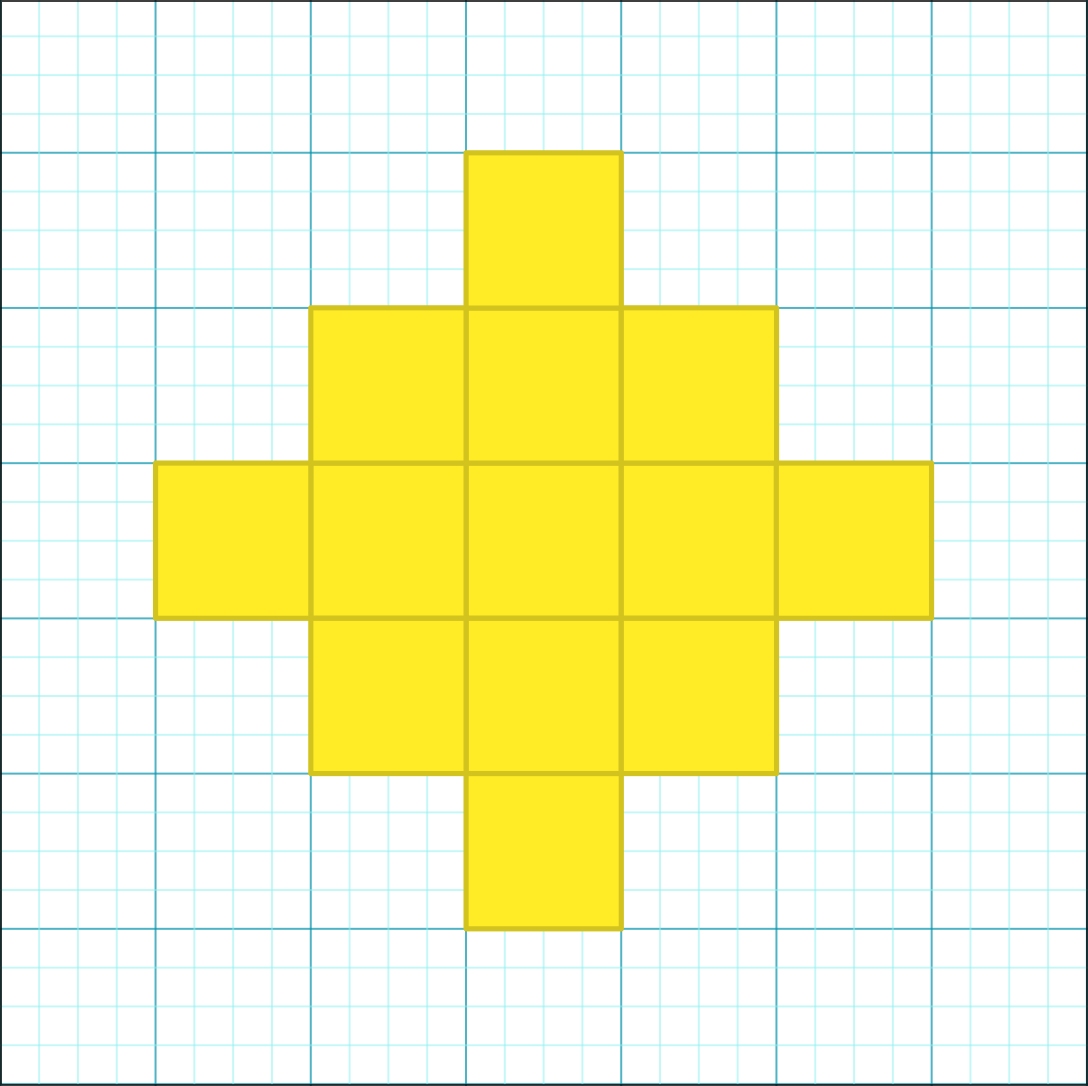
\includegraphics[width=0.3\textwidth]{example.png}
    \caption{Example du sample 1}
\end{figure}


\begin{Input}
    L'input consiste en une seule ligne avec un entier $n$ ($0\leq n\leq \maxn$), le nombre de bac.
\end{Input}

\begin{Output}
    Un entier représentant la taille maximale de l'étoile.
\end{Output}
